\chapter{Технологический раздел}
В данном разеделе представлены требование к ПО, выбор инструментов для реализации и оценки алгоритмов, а также листинги полученного кода.

\section{Требование к ПО}

К программе предъявляется ряд требований:

\begin{itemize}
	\item на вход подаётся строка;
	\item на выходе — самый длинный полиндром, если таких несколько, то первый в строке.
\end{itemize}

\section{Выбор инструментов}
Поскольку наиболее освоенным языком для разработчика является c++, для реализации поставленной задачи был выбран именно он, т.к. таким образом работа будет проделана наиболее быстро и качественно.

Соответственно для компиляции кода будет использоваться компилятор G++.

Чтобы оценить время выполнения программы, будет замерятся реальное время, т.к. таким образом можно будет сравнить реализацию с конвейером и без. Для замера реального времени работы программы используется функция $chrono::high\_resolution\_clock::now()$ т.к. программа апробируется на компьютере с установленной ОС Windows. \cite{chrono()}

Кроме этого, необходимо отключить оптимизации компилятора для более честного сравнения алгоритмов. В моём случае это делается с помощью ключа $-O0$ т.к. используется компилятор G++. \cite{optimization}

\section{Реализация алгоритмов}
На листингах \ref{Conveyor::process}-\ref{conveer3} представлены реализации алгоритма работы для главного потока и реализации алгоритмов лент конвейера.

\begin{lstinputlisting}[
	caption={Реализация алгоритма работы для главного потока},
	label={Conveyor::process},
	style={c},
	]{inc/src/process.c}
\end{lstinputlisting}

\newpage
\begin{lstinputlisting}[
	caption={Реализация алгоритма первой ленты конвейера},
	label={conveer1},
	style={c},
	linerange={1-25},
	]{inc/src/conveer.c}
\end{lstinputlisting}

\newpage
\begin{lstinputlisting}[
	caption={Реализация алгоритма второй ленты конвейера},
	label={conveer2},
	style={c},
	linerange={27-51},
	]{inc/src/conveer.c}
\end{lstinputlisting}

\newpage
\begin{lstinputlisting}[
	caption={Реализация алгоритма третьей ленты конвейера},
	label={conveer3},
	style={c},
	linerange={53-79},
	]{inc/src/conveer.c}
\end{lstinputlisting}

\section{Тестирование}
Для проверки написанных алгоритмов были подготовлены следующие тесты:
\begin{itemize}
	\item проверка реузльтата обработки строки "test lol 23323232 s sss ll 2332323322 sls sll lls"
	\item проверка реузльтата обработки строки "test lol 23323232 s sss ll 233232332 sls sll lls"
	\item проверка реузльтата обработки строки "te str"
\end{itemize}

Для подготовленных тестов ожидаются следующие результаты соответсвтенно:
\begin{itemize}
	\item "lol"
	\item "233232332"
	\item "No polinoms"
\end{itemize}

На рисунке \ref{tests} приведены результаты тестирования. Тестирование проводилось по методу чёрного ящика.

%\newline
\begin{figure}[h]
	\center{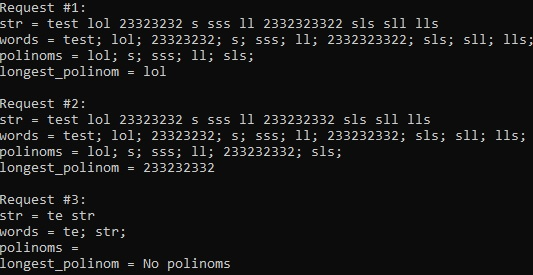
\includegraphics[width=1\linewidth]{inc/img/tests}}
	\caption{Результаты тестирования}
	\label{tests}
\end{figure}

Как видно, все тесты пройдены.

\section{Вывод}
В данном разделе были выдвинуты требования к ПО, выбраны инструменты для реализации выбранных алгоритмов, представлены листинги реализованных алгоритмов, а также проведено тестирование.